\documentclass[12pt,a4paper]{article}
\usepackage{fullpage}
\usepackage[margin=2cm]{geometry}
\usepackage{amsmath}
\usepackage{subfig}
\usepackage{graphicx}
\usepackage[justification=centering]{caption}
\begin{document}
\title{Fine-tuning trained models on pronotum datasets}
\author{LE Van Linh}
\date{\today}
\maketitle
\begin{abstract}
	In this study, we fine-tune on the trained models on pronotum dataset, such as VGG16, VGG19, VGG-CNNS, and ResNet50. Most of the models are Convolutional Neural Networks (CNN) for classification problems. They are trained on ImageNet database. After training, the models are able to classify $1000$ classes as the output. To study how does a network which was designed for classification problem work on regression problem, we fine-tune the trained model on pronotum dataset. The experiments will implement on two steps: freeze and unfreeze some layers in trained models. At the end of the experiment, a comparison between the fine-tune losses will be discussed.
\end{abstract}
\section{Dataset}
The dataset includes 293 RGB-images of beetle's pronotum. The images were taken by the same camera with the same conditions of resolution of $3264 \times 2448$. The images in the dataset were divided into two subsets: training (including $260$ images) and testing (including $33$ images). For each image, a set of 8 manual landmarks have been set by biologists. Depending the input of the pre-trained models, the images are down-sampled to fit with the models. Firstly, the images are down-sampled to a resolution of $326 \times 245$ and the coordinates of the manual landmarks are also re-scaled. Secondly, the centroid point of manual landmarks is calculated for each image. The centroid point is considered as the center of the new image that has been cropped from the down-sampled image. The size of the new image is depending on the input of the trained model that we would like to fine tune. Fig. \ref{figdata} presents an example in dataset after down-sampling and crop the image to fit with the input size of neural network.

\begin{figure}[h!]
\centering
\subfloat[]{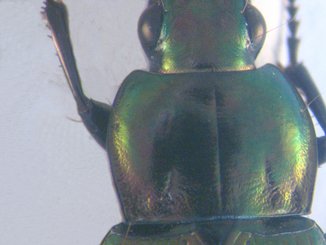
\includegraphics[scale=1.1]{./images/imagenet_finetuning/Prono_001_326}\label{a1}}\hspace{1cm}
\subfloat[]{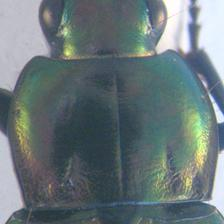
\includegraphics[scale=0.5]{./images/imagenet_finetuning/Prono_001_224}{\label{a2}}}
\caption{An example in dataset. \textit{a)} presents the image after down-sampling. \textit{b)} presents the cropped image from down-sampling image which used as the input of CNN}
\label{figdata}
\end{figure}
\section{The models}
\subsection{VGGs models}
The models are the improved versions of the models used by the VGG team in ILSVRC-2014 competition \cite{simonyan2014very}. The models were designed to evaluate the depth of the network by using an architecture with very small ($3 \times 3$) convolution filters and pushing the depth to $16 \to 19$ weight layers. Table. shows the architecture of the VGGs models.

\begin{table}[h!]
	\centering
	\begin{tabular}{c l l l}
	Layer & $VGG-16$ & $VGG-19$ & $VGG-CNNS$ \\ \hline
	0 & Input(3,224,224) & Input(3,224,224) & \\ \hline
	1 & CONV(64,3,1) & CONV(64,3,1) & \\ \hline
	2 & CONV(64,3,1) & CONV(64,3,1) & \\ \hline
	3 & POOL(2) &  POOL(2) & \\ \hline
	4 & CONV(128,3,1) & CONV(128,3,1) & \\ \hline
	5 & CONV(128,3,1) & CONV(128,3,1) & \\ \hline
	6 & POOL(2) &  POOL(2) & \\ \hline
	7 & CONV(256,3,1) & CONV(256,3,1) & \\ \hline
	8 & CONV(256,3,1) & CONV(256,3,1) & \\ \hline
	9 & CONV(256,3,1) & CONV(256,3,1) & \\ \hline
	10 & POOL(2) &  CONV(256,3,1) & \\ \hline
	11 & CONV(512,3,1) & POOL(2) & \\ \hline
	12 & CONV(512,3,1) & CONV(512,3,1) & \\ \hline
	13 & CONV(512,3,1) & CONV(512,3,1) & \\ \hline
	14 & POOL(2) &  CONV(512,3,1) & \\ \hline
	15 & CONV(512,3,1) & CONV(512,3,1) & \\ \hline
	16 & CONV(512,3,1) & POOL(2) & \\ \hline
	17 & CONV(512,3,1) & CONV(512,3,1) & \\ \hline
	18 & POOL(2) &  CONV(512,3,1) & \\ \hline
	19 & FC(4096) & CONV(512,3,1)  &\\ \hline
	20 & DROP(0.5) & CONV(512,3,1)  &\\ \hline
	21 & FC(4096) & POOL(2)  &\\ \hline
	22 & DROPOUT(0.5) &  FC(4096) & \\ \hline
	23 & FC(1000) & DROP(0.5) & \\ \hline
	24 & - & FC(4096)  &\\ \hline
	25 & - &  DROP(0.5)  &\\ \hline
	26 & - &  FC(1000)  &\\ \hline
	\end{tabular}
	\caption{The architecture of VGG-16,VGG-19, and VGG-CNN-S}
	\label{VGGmodels}
\end{table}

\subsection{ResNet50 model}
ResNet50\cite{he2015deep} was designed as a residual learning framework to ease the training of networks. The network had a depth of up to $152$ layers---$8$x deeper than VGG networks. An ensemble of these residual nets achieves $3.57\%$ error on the ImageNet test set. This result won the 1st place on the ILSVRC 2015 classification task.

The parameters which used to setup the network during fine-tuning, have been shown in Table.\ref{model2parameters}. These parameters of every fine-tuning process are the same.
\begin{table}[h!]
	\centering
	\begin{tabular}{l l l}
	Parameter & Initial value & End value \\ \hline
	Epochs & 5000 &  \\ \hline
	Training batch size & 128 & \\ \hline
	Testing batch size & 128 & \\ \hline
	Learning rate & 0.000001 &  \\ \hline
	Momentum & 0.9 &  \\ \hline
	\end{tabular}
	\caption{The network parameters in fine-tuning model}
	\label{model2parameters}
\end{table}
\section{Experiments}
The dataset includes 260 image in 3-channels was used to fine-tune on each trained model. Table.\ref{result} shows the losses during fine-tuning (training and validation loss). During fine-tuning, the learning rate and momentum were kept the same on all trained model ($0.000001$ and $0.9$, respective). Each model was fine-tuned in two steps: \textit{freeze and un-freeze} some ``lower" layers in $5000$ epochs.

\begin{table}[h!]
	\centering
	\begin{tabular}{l l l}
	Model & Training loss & Validation loss \\ \hline
	VGG-16 (unfreeze) & 11.00030 & 9.41890  \\ \hline
	VGG-16 (freeze) & 12.52632 & 12.75353 \\ \hline
	VGG-19 (unfreeze) & 10.90212 & 8.58467 \\ \hline
	VGG-19 (freeze) & 11.00235 & 9.29593 \\ \hline
	VGG-CNNS (unfreeze) & 8.56958 & 13.49900 \\ \hline
	VGG-CNNS (freeze) & 8.42673 & 13.41841 \\ \hline
	ResNet (unfreeze) & 0.05461 & 115.05157 \\ \hline
	ResNet (freeze) & 0.04200 & 122.41291 \\ \hline
	\end{tabular}
	\caption{The losses during fine-tuning the trained models}
	\label{result}
\end{table}
From the losses in Table.\ref{result}, the classification models can be used to fine-tune on a regression problem. However, the result seems that not good as we expect. Besides, to ensure the fine-tuning work, the learning rate have been set to a very small value ($0.000001$). This will spend a lot of time for fine-tuning. The lowest of validation value is $sqrt(8.58467) \approx 2.929$.

In the list of result, the train loss of ResNet is very impressive but the range between training and validation is very large. This problem appears as an overfitting on this model.
\section{Conclusions}
In this study, we have fine-tuned some trained models on pronotum dataset (RGB format). All the models have been worked well for a regression problem. Despite, the efficiencies of fine-tuning processes are not good enough as we expect. Besides, the limitation of data had overfitting reappear.
\bibliographystyle{unsrt}
\bibliography{includes/references}

\end{document}